\section[Basic Statistics Examples]{Basic Statistics Examples}

\label{sec:statistics_examples}
\addcontentsline{toc}{section}{\thesection. Basic Statistics Examples}

This section introduces four simple examples and explains a little about computing with 
distributed data. 
These implemented examples/functions are partly
selected from the Cookbook of HPSC website~\citep{hpsc2011} at
\url{http://thirteen-01.stat.iastate.edu/snoweye/hpsc/?item=cookbook}.
Please see more details there.

\subsection[Monte Carlo Simulation]{Monte Carlo Simulation}
\label{sec:monte_carlo}
\addcontentsline{toc}{subsection}{\thesubsection. Monte Carlo Simulation}

The demo command is
\begin{Command}
### At the shell prompt, run the demo with 4 processors by
### (Use Rscript.exe for windows system)
mpiexec -np 4 Rscript -e "demo(monte_carlo,'pbdDEMO',ask=F,echo=F)"
\end{Command}

This is a simple Monte Carlo simulation example for numerically estimating $\pi$.
Suppose we sample $N$ uniform observations $(x_i, y_i)$ inside (or perhaps on the border of) the unit square $(0, 1)\times (0,1)$,
where $i = 1, 2, \ldots, N$.  Then
\begin{equation}
\pi \approx 4\frac{L}{N}
\label{eqn:pi}
\end{equation}
where $0\leq L\leq N$ is the number of observations sampled satisfying
\begin{align*}
x_i^2+y_i^2 \leq 1
\end{align*}
The intuitive explanation for this is strategy which is sometimes given belies a misunderstanding of infinite cardinalities, and infinite processes in general.  We are not \emph{approximating} an area, because to do so with points would be madness requiring a transfinite process.  

In reality, we are evaluating the probability that someone throwing a 0-dimensional ``dart'' at the unit square will have that ``dart'' also land below the arc of the unit circle contained within the unit square.  Formally, let $U_1$ and $U_2$ be random uniform variables, each from the closed unit interval $[0, 1]$.  Define the random variable
\begin{align*}
X &:= 
\begin{cases} 
1\text{, } \hspace{.4cm} U_1^2 + U_2^2 \leq 1\\ 
0\text{, \hspace{.4cm} otherwise}
\end{cases}
\end{align*}
Let $V_i = U_i^2$ for $i=1, 2$. Then the expected value
\begin{align*}
E[X] &= P( V_1 + V_2 \leq 1 )\\
     &= \int_0^1 \int_0^{1-V_1} p(V_1, V_2)dV_2 dV_1\\
     &= \int_0^1 \int_0^{1-V_1} \left( \frac{1}{2\sqrt{V_1}} \right) \left( \frac{1}{2\sqrt{V_2}} \right)dV_2 dV_1\\
     &= \frac{1}{2}\int_0^1 \left(\frac{1-V_1}{V_1}\right)^{1/2}dV_1\\
     &= \frac{1}{2} \left[ 
	V_1\left(\frac{1-V_1}{V_1}\right)^{1/2} 
	 - \frac{1}{2} \arctan\left(\frac{\left(\frac{1-V_1}{V_1}\right)^{1/2} (2V_1-1)}{2(V_1-1)}\right) 
	\right]_{V_1\rightarrow 0}^{V_1\rightarrow 1}\\
     &= \frac{1}{2}\left[ \frac{\pi}{4} +\frac{\pi}{4}  \right]
\end{align*}
and by sampling observations $X_i$ for $i=1,\dots,N$, by the Strong Law of Large Numbers
\begin{align*}
\bar{X}_N \longrightarrow^{\hspace{-.55cm} a.s.} \hspace{.1cm} \frac{\pi}{4} \hspace{.4cm} \text{ as } N\rightarrow \infty
\end{align*}
In other words,
\begin{align*}
P\left(\lim_{N\rightarrow\infty} \bar{X}_N = \frac{\pi}{4}\right) = 1
\end{align*}
Whence,
\begin{align*}
\frac{L}{N}  \longrightarrow^{\hspace{-.55cm} a.s.} \hspace{.1cm} \frac{\pi}{4} \hspace{.4cm} \text{ as } N\rightarrow \infty
\end{align*}

But because no one is going to read that, and if they do they'll just call me a grumpy old man,
\begin{figure}[h]
 \centering
 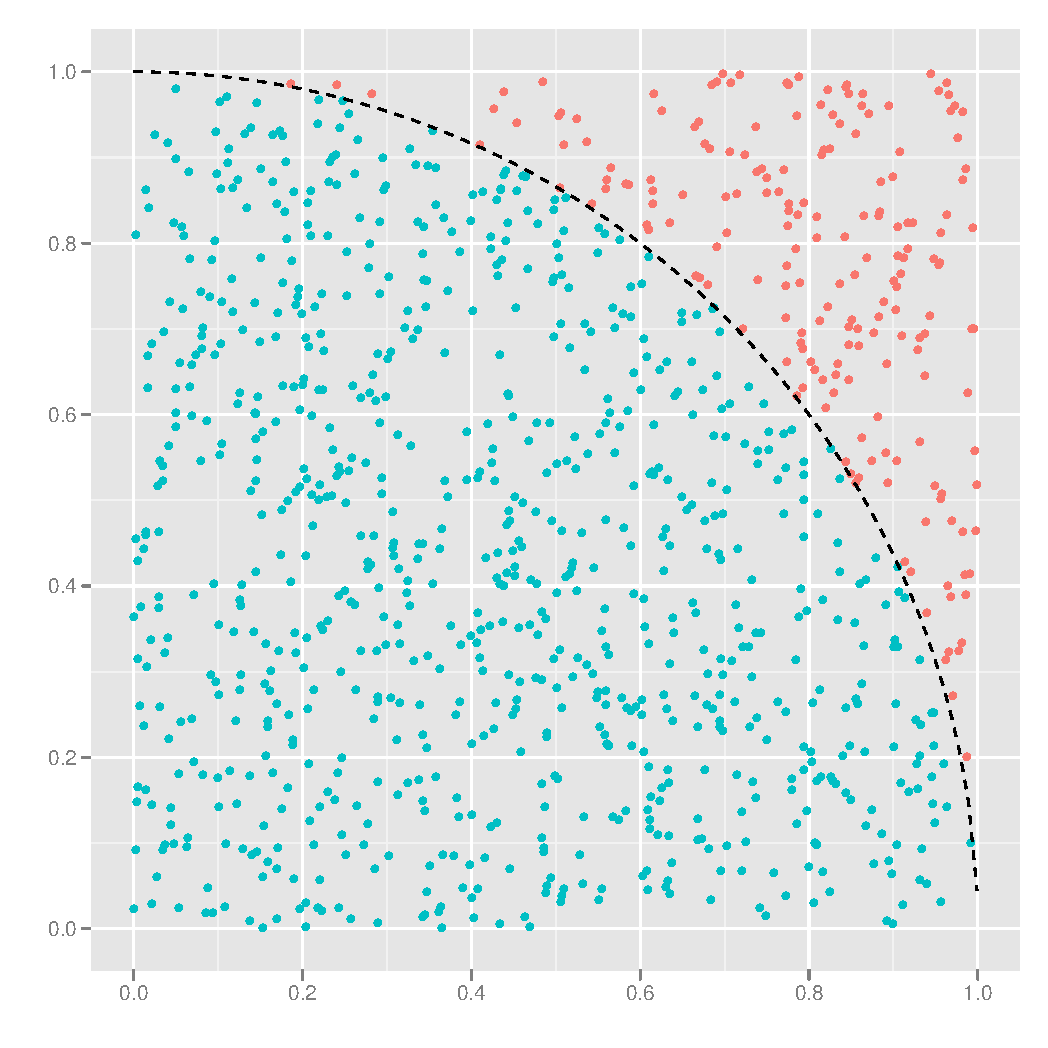
\includegraphics[height=8.5cm, width=8.5cm]{pbdDEMO-include/pics/misleading}
 \caption{Approximating $\pi$ by Monte Carlo methods}\label{pic:dumb}
\end{figure}
 the misleading picture you desire can be found in Figure~\ref{pic:dumb}.



The key step of the demo code is in the following block:
\begin{lstlisting}[language=rr,title=R Code]
N.spmd <- 1000
X.spmd <- matrix(runif(N.spmd * 2), ncol = 2)
r.spmd <- sum(rowSums(X.spmd^2) <= 1)
ret <- allreduce(c(N.spmd, r.spmd), op = "sum")
PI <- 4 * ret[2] / ret[1]
comm.print(PI)
\end{lstlisting}

In line 1, we specify sample size in \code{N.spmd} for each processor,
and $N=D\times\mbox{\code{N.spmd}}$ if $D$ processors are executed.
In line 2, we generate samples in \code{X.spmd} for every processor.
In line 3, we compute how many of radios are less than or equal to $1$
for each processors.
In line 4, we call \code{allreduce} to obtain total numbers across all
processors.
In line 5, we use the Equation~(\ref{eqn:pi}).
Since SPMD, \code{ret} is common on all processors, and so is \code{PI}.




\subsection[Sample Mean and Sample Variance]{Sample Mean and Sample Variance}
\label{sec:sample_stat}
\addcontentsline{toc}{subsection}{\thesubsection. Sample Mean and Sample Variance}

The demo command is
\begin{Command}
### At the shell prompt, run the demo with 4 processors by
### (Use Rscript.exe for windows system)
mpiexec -np 4 Rscript -e "demo(sample_stat,'pbdDEMO',ask=F,echo=F)"
\end{Command}

Suppose $\bx = \{x_1, x_2, \ldots, x_N\}$
are observed samples, and $N$ is potentially very large.
We can distribute $\bx$ in 4 processors, and each processor receives a proportional amount of data. One simple way to compute sample mean $\bar{x}$ and
sample variance $s_x$ is based on the formulas:

\begin{align}
\bar{x} &= \frac{1}{N} \sum_{n = 1}^N x_n \notag \\[.3cm]
        &= \sum_{n = 1}^N \frac{x_n}{N} \label{math:mn}
\end{align}
and
\begin{align}
s_x     &= \frac{1}{N - 1} \sum_{n = 1}^N (x_n - \bar{x})^2 \notag \\[.3cm]
        &= \frac{1}{N - 1} \sum_{n = 1}^N x_n^2 - \frac{2\bar{x}}{N - 1}\sum_{n = 1}^N x_n +  \frac{1}{N - 1}\sum_{n = 1}^N\bar{x}^2 \notag \\[.3cm]
        &= \sum_{n = 1}^N \left(\frac{x^2_n}{N-1}\right) - \frac{N \bar{x}^2}{N-1} \label{math:sd}
\end{align}
where expressions (\ref{math:mn}) and (\ref{math:sd}) are one-pass algorithms,
which are potentially faster and more stable than the first expressions,
especially for large $N$. Here, only the first and second moments are implemented, while
the extension of one-pass algorithms to higher order moments is also
possible.

The demo command is
\begin{Command}
### At the shell prompt, run the demo with 2 processors by
### (Use Rscript.exe for windows system)
mpiexec -np 2 Rscript -e "demo(sample_stat,'pbdDEMO',ask=F,echo=F)"
\end{Command}

The demo \code{sample_stat} generates fake data on 2 processors, then
utilize \code{mpi.stat} function as

The demo \code{sample_stat} generates fake data on 4 processors, then
utilizes \code{mpi.stat} function as
\begin{lstlisting}[language=rr,title=R Code]
mpi.stat <- function(x.spmd){
  ### For mean(x).
  N <- allreduce(length(x.spmd), op = "sum")
  bar.x.spmd <- sum(x.spmd / N)
  bar.x <- allreduce(bar.x.spmd, op = "sum")

  ### For var(x).
  s.x.spmd <- sum(x.spmd^2 / (N - 1))
  s.x <- allreduce(s.x.spmd, op = "sum") - bar.x^2 * (N / (N - 1))

  list(mean = bar.x, s = s.x)
} # End of mpi.stat().
\end{lstlisting}
where \code{allreduce} in \pkg{pbdMPI}~\citep{Chen2012pbdMPIpackage} can
be utilized in this examples to aggregate local information across
all processors.

\subsection[Binning]{Binning}
\label{sec:binning}
\addcontentsline{toc}{subsection}{\thesubsection. Binning}

The demo command is
\begin{Command}
### At the shell prompt, run the demo with 4 processors by
### (Use Rscript.exe for windows system)
mpiexec -np 4 Rscript -e "demo(binning,'pbdDEMO',ask=F,echo=F)"
\end{Command}

Binning is a classical statistics and can quickly summarize
the data structure by setting some breaks between max and min of data.
This is particularly a useful tool for constructing histograms and
categorical data analysis.

The demo \code{binning} generates fake data on 4 processors, then
utilize \code{mpi.bin} function as
\begin{lstlisting}[language=rr,title=R Code]
mpi.bin <- function(x.spmd, breaks = pi / 3 * (-3:3)){
  bin.spmd <- table(cut(x.spmd, breaks = breaks))
  bin <- as.array(allreduce(bin.spmd, op = "sum"))
  dimnames(bin) <- dimnames(bin.spmd)
  class(bin) <- class(bin.spmd)
  bin
} # End of mpi.bin().
\end{lstlisting}
An easy implementation is to utilize \code{table} function to obtain
local counts, then call \code{allreduce} to obtain global counts.



\subsection[Quantile]{Quantile}
\label{sec:quantile}
\addcontentsline{toc}{subsection}{\thesubsection. Quantile}

The demo command is
\begin{Command}
### At the shell prompt, run the demo with 4 processors by
### (Use Rscript.exe for windows system)
mpiexec -np 4 Rscript -e "demo(quantile,'pbdDEMO',ask=F,echo=F)"
\end{Command}

Quantile is the other useful tool from fundamental statistics
which provides data distribution for the desired value.
This example can be extended to construct Q-Q plot,
compute cumulative density function and nonparametric statistics,
solve maximum likelihood estimators.

This is only an inefficient implementation to approximate a quantile
and is not equivalent to the original \code{quantile} function in
\proglang{R}. But in some sense, it should work well in large scale.
The demo \code{quantile} generates fake data on 4 processors, then
utilizes \code{mpi.quantile} function as
\begin{lstlisting}[language=rr,title=R Code]
mpi.quantile <- function(x.spmd, prob = 0.5){
  if(sum(prob < 0 | prob > 1) > 0){
    stop("prob should be in (0, 1)")
  }

  N <- allreduce(length(x.spmd), op = "sum")
  x.max <- allreduce(max(x.spmd), op = "max")
  x.min <- allreduce(min(x.spmd), op = "min")

  f.quantile <- function(x, prob = 0.5){
    allreduce(sum(x.spmd <= x), op = "sum") / N - prob
  }

  uniroot(f.quantile, c(x.min, x.max), prob = prob[1])$root
} # End of mpi.quantile().
\end{lstlisting}
where a numerical function is solved by \code{uniroot} to find out
the appropriate value such that cumulated probability is less than
or equal to the specified quantile.

This simple example shows that the SPMD is greatly applicable on large
scale data analysis and likelihood computing.
Note that the \code{uniroot} call is working in parallel and on distributed
data, i.e. other optimization functions such as \code{optim} and \code{nlm}
can be utilized in the same way,
since SPMD simply assumes every processors do the same work
simulatinuously.




\subsection[Ordinary Least Squares]{Ordinary Least Squares}
\label{sec:ols}
\addcontentsline{toc}{subsection}{\thesubsection. Ordinary Least Squares}

The demo command is
\begin{Command}
### At the shell prompt, run the demo with 4 processors by
### (Use Rscript.exe for windows system)
mpiexec -np 4 Rscript -e "demo(ols,'pbdDEMO',ask=F,echo=F)"
\end{Command}

Ordinary least squares (OLS)
is perhaps \emph{the} fundamental tool of the statistician.  The goal is to find a solution $\bbeta$ such that
\begin{align}
\ltwo{ \bX\bbeta - \by }^2 \label{math:lls}
\end{align}
which is minimized.  In statistics, we tend to prefer to think of the problem as being of the form
$$\by = \bX\bbeta + \bepsilon$$
where $\by$ is $N\times 1$ observed vector,
$\bX$ is $N\times p$ designed matrix which is full rank and $N >> p$,
$\bbeta$ is the insterested parameters and unknown to be estimated,
and $\bepsilon$ is errors and to be minimized in norm.

Note that above, we do indeed mean (in fact, stress) \emph{a} solution to the linear least squares problem.  The full story is somewhat complicated.  The short explanation is that for many applications a statistician will face, expression (\ref{math:lls}) will actually have a unique solution.  But this is not always the case.  Indeed, it may occur that there is an infinite family of solutions.  So typically we go further and demand that a solution $\bbeta$ be such that $\ltwo{\bbeta}$ is at least as small as the corresponding norm of any other solution (although even this does not guarantee uniqueness).

A properly thorough treatment of the problems involved here go beyond the scope of this document, and require the reader have in-depth familiarity with linear algebra.  For our purposes, the concise explanation above will suffice.

The classical Maximum Likelihood solution is given by:
\begin{align}
 \hat{\bbeta} = (\bX^t\bX)^{-1}\bX^t\by \label{math:ols}
\end{align}
 
This example can be also generalized to weighted least square (WLS),
and linear mixed effect models (LME).

The implementation is straight forward as
\begin{lstlisting}[language=rr,title=R Code]
mpi.ols <- function(y.spmd, X.spmd){
  if(length(y.spmd) != nrow(X.spmd)){
    stop("length(y.spmd) != nrow(X.spmd)")
  }

  t.X.spmd <- t(X.spmd)
  A <- allreduce(t.X.spmd %*% X.spmd, op = "sum")
  B <- allreduce(t.X.spmd %*% y.spmd, op = "sum")

  solve(matrix(A, ncol = ncol(X.spmd))) %*% B
} # End of mpi.ols().

\end{lstlisting}

While this is a fine demonstration of the power of ``getting your hands dirty'', this approach is only efficient for small $N$ and small $p$.  Worse, directly computing the product
\begin{align*}
\bX^t\bX
\end{align*}
is often numerically non-stable.  Instead, it is generally better (although much slower) to take an orthogonal factorization of the data matrix.  Typically, the QR-decomposition is used to this end.  Here $\bX=QR$, where $Q$ is orthogonal and $R$ is upper trapezoidal.  This is beneficial, because orthogonal matrices are norm-preserving, and whence
\begin{align*}
\ltwo{\bX\bbeta - \by} &= \ltwo{QR\bbeta - \by}\\
  &= \ltwo{Q^TQR\bbeta - Q^T\by}\\
  &= \ltwo{R\bbeta - Q^T\by}
\end{align*}
The (arguably) much more well-known Singular Value Decomposition can also be used to develop yet another algebraically identical solution which is quite elegant.  Here, if we take $\bX = U\Sigma V^T$, then it can be shown that ``the'' desired solution is given by
\begin{align*}
\bbeta = V\Sigma^+ U^T\by
\end{align*}
where $\Sigma^+$ is the Moore-Penrose pseudoinverse of $\Sigma$.  However, this approach is handily the most computationally intensive.

The method utilizing QR to find a minimum norm solution has been implemented in \pkg{pbdDMAT} for objects of class \code{ddmatrix}.  For larger problems, and especially those where numerical accuracy is important, it may be more convenient to simply convert \code{y.spmd} and \code{X.spmd} into block-cyclic format as in the Part~\ref{part:dmat} and
to utilize \pkg{pbdBASE} and \pkg{pbdDMAT} for all matrix computation.

